\subsection{UC17 - Visualizzazione Riunioni Giornaliere }
\begin{itemize}
	\item \textbf{Identificativo}: UC17
	\item \textbf{Nome}: Visualizzazione Riunioni Giornaliere
	\item\textbf{Descrizione Grafica}: 
	\begin{center}
		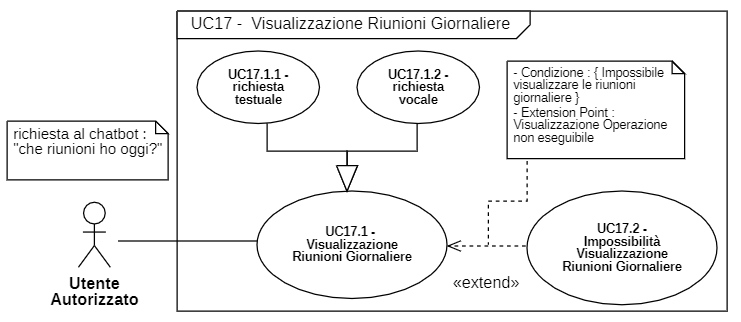
\includegraphics[scale=0.65]{images/UC17.png} 
	\end{center}

	\item \textbf{Attori}
	\begin{itemize} 
		\item \textit{Primari}: Utente autorizzato e autenticato nella \glossario{piattaforma riunioni}
		\item \textit{Secondari}: Non presenti
	\end{itemize}
	\item \textbf{Descrizione}: L'utente richiede di visualizzare le Riunioni del giorno.
	\item \textbf{Precondizione}: L'utente ha effettuato il login sia sull'app che sulla piattaforma esterna, e si trova nella chat.
	\item \textbf{Postcondizione}: Il chatbot restituisce la lista delle riunioni del giorno, con eventuali informazioni.
	\item \textbf{Scenario principale}:  \begin{enumerate}
		\item Utente invia un messaggio al chatbot : "Che riunioni ho oggi?";
		\item Chatbot restituisce la lista delle riunioni, con eventuali informazioni.
	\end{enumerate}
\end{itemize}